\documentclass[12pt]{article}      
\usepackage{epsfig,multirow,setspace}

\AtEndOfClass{\RequirePackage{times}}
\textwidth=165mm \headheight=0mm \headsep=10mm \topmargin=0mm
\textheight=210mm %\footskip=1.5cm
\oddsidemargin=0mm
% Any additional packages needed should be included after jmlr2e.
% Note that jmlr2e.sty includes epsfig, amssymb, natbib and graphicx,
% and defines many common macros, such as 'proof' and 'example'.
%
% It also sets the bibliographystyle to plainnat; for more information on
% natbib citation styles, see the natbib documentation, a copy of which
% is archived at http://www.jmlr.org/format/natbib.pdf

%\usepackage{jmlr2e}
\usepackage{mathtools}
\usepackage{amsthm,amsmath,amssymb,colonequals,multirow,graphicx,epstopdf}
\usepackage{caption}
\usepackage{color}
\usepackage{mwe}
%\usepackage{colonequals}a
% Definitions of handy macros can go here

\usepackage[caption=false,font=footnotesize,labelfont=sf,textfont=sf]{subfig}
\usepackage{fancyhdr}
\usepackage{amsfonts, amsmath, amssymb, marvosym, upgreek, mathrsfs, dsfont} 
\usepackage{array,graphicx}
\usepackage{booktabs}
\usepackage{pifont}
\usepackage{setspace}
\usepackage{colonequals} 
\usepackage[authoryear]{natbib}

\renewcommand\harvardyearleft{\unskip, }
\renewcommand\harvardyearright[1]{.}
\newcommand\Fontvi{\fontsize{8}{7.2}\selectfont}
\newcommand{\vecX}{\mathbf{X}}
\newcommand{\vecZ}{\mathbf{Z}}
\newcommand{\vecU}{\mathbf{U}}
\newcommand{\vecI}{\mathbf{I}}
\newcommand{\vecO}{\mathbf{O}}
\newcommand{\vecE}{\mathbf{E}}
\newcommand{\vecM}{\mathbf{M}}
\newcommand{\vecS}{\mathbf{S}}
\newcommand{\vecT}{\mathbf{T}}
\newcommand{\vecx}{\mathbf{x}}
\newcommand{\vecu}{\mathbf{u}}
\newcommand{\vecz}{\mathbf{z}}
\newcommand{\veczero}{\mathbf{0}}
\newcommand{\vecmu}{\mbox{\boldmath$\mu$}}
\newcommand{\veczeta}{\mbox{\boldmath$\zeta$}}
\newcommand{\vecalpha}{\mbox{\boldmath$\alpha$}}
\newcommand{\vecbeta}{\mbox{\boldmath$\beta$}}
\newcommand{\vecgamma}{\mbox{\boldmath$\gamma$}}
\newcommand{\veclambda}{\mbox{\boldmath$\lambda$}}
\newcommand{\vecLambda}{\mbox{\boldmath$\Lambda$}}
\newcommand{\vecomega}{\mbox{\boldmath$\omega$}}
\newcommand{\vecpi}{\mbox{\boldmath$\pi$}}
\newcommand{\matsig}{\mbox{\boldmath$\Sigma$}}
\newcommand{\matTheta}{\mbox{\boldmath$\Theta$}}
\newcommand{\matepsilon}{\mbox{\boldmath$\epsilon$}}
\newcommand{\matPsi}{\mbox{\boldmath$\Psi$}}
\newcommand{\varthet}{\mbox{\boldmath$\vartheta$}}
\newcommand{\ttr}{\text{tr}}
\newcommand{\iprod}{\prod_{i=1}^n}
\newcommand{\isum}{\sum_{i=1}^n}
\newcommand{\gsum}{\sum_{g=1}^G}
\newcommand{\inv}{^{\raisebox{.2ex}{$\scriptscriptstyle-1$}}}
\DeclareMathOperator{\E}{\mathbb{E}}
\DeclareMathOperator{\R}{\mathbb{R}}
\newtheorem{prop}{Proposition}
\hyphenation{McNicholas}


\begin{document}

\title{Finite Mixtures of Multivariate Poisson-Log Normal Factor Analyzers for Clustering Count Data}

\author{Anjali Silva\footnote{Department of Mathematics and Statistics, University of Guelph, Guelph, ON, Canada.}\qquad\qquad\qquad Steven~J.~Rothstein\footnote{Department of Molecular and Cellular Biology, University of Guelph, Guelph, ON, Canada.}\\\hspace{-0.4in}Paul~D.~McNicholas\footnote{Department of Mathematics and Statistics, McMaster University, Hamilton, ON, Canada.} \qquad\qquad Sanjeena Subedi\footnote{Department of Mathematical Sciences, Binghamton University, Binghamton, New York, USA.}}
\date{}

\maketitle

%%%%%%Abstract%%%%%%%
\begin{abstract}
A mixture of multivariate Poisson-log normal factor analyzers is introduced by imposing constraints on the covariance matrix, which resulted flexible models for clustering purposes. In particular, a class of four parsimonious mixture models based on the mixtures of factor analyzers model are introduced. A Markov chain Monte Carlo alternating expectation-conditional maximization algorithm (MCMC-AECM) is used for model parameter estimation, and information criteria are used for model selection. The proposed models are explored in the context of clustering discrete data arising from RNA sequencing studies. Using real and simulated data, the models are shown to give favorable clustering performance.
\end{abstract}

%%%%%%Introduction%%%%%%
\section{Introduction}\label{sec:intro}
Model-based clustering is a technique that utilizes finite mixture models to cluster data  \citep{wolfe1965, mclachlanandbasford1998, mclachlan2000, mcnicholas2016}. The general distribution function for mixture models can be given as $f( \mathbf{y}| \pi_1, \ldots, \pi_G,\boldsymbol{\vartheta}_1, \ldots, \boldsymbol{\vartheta}_G )$ $= \sum_{g=1}^{G} \pi_g f_g( \mathbf{y} | \boldsymbol{\vartheta}_g)$, where $G$ is the total number of clusters, $f_g(\cdot)$ is the distribution function with parameters $\boldsymbol{\vartheta}_g$, and $ \pi_g>0$ is the mixing weight of the $g^{\text{th}}$ component such that $\sum_{g=1}^G\pi_g=1$. Mixture model-based clustering methods can be over-parameterized in high-dimensional spaces, especially as the number of clusters increases. Subspace clustering allows to cluster data in low-dimensional subspaces, while keeping all the dimensions and by introducing restrictions to mixture parameters \citep{bouveyron2012}. Restrictions are introduced to the model parameters with the aim of obtaining parsimonious models, which are sufficiently flexible for clustering purposes. 

The factor analysis model by \citet{spearman1904} assumes that a $p$-dimensional vector of observed variables, $\mathbf{\vecX}$, can be modeled by a $q$-dimensional vector of latent factors, where $q \textless p$. As a result, the factor analysis model is useful in modeling the covariance structure of high-dimensional data using a small number of latent variables. The mixture of factor analyzers model was later introduced \citep{ghahramani1997} and this model is able to concurrently perform clustering and, within each cluster, local dimensionality reduction. Consider $n$ independent $p$-dimensional continuous variables $\vecX_1, \ldots, \vecX_n$, which come from a heterogeneous population with $G$ subgroups. In mixture of factor analyzers framework, $\vecX_i$ is modelled as
\begin{equation*}
\vecX_i = \vecmu_g + \vecLambda_g\vecU_{ig}+ \matepsilon_{ig},
\end{equation*} 
for $i=1,\ldots,n$ and $g=1,\ldots,G$. Here, $\vecmu_g$ is a $p \times 1$ vector of $g$th component mean, $\vecLambda_g$ is a $p \times q$ matrix of $g$th component factor loadings, $\vecU_{ig} \sim \mathcal{N}_q(\veczero,\vecI_q)$ is a $q \times 1$ vector of $g$th component latent factors, and $\matepsilon_{ig}\sim\mathcal{N}_p(\veczero,\matPsi_g)$ is a $p \times 1$ vector of $g$th component errors with $\matPsi_g = \text{diag}(\psi_{g1},\ldots,\psi_{gp})$. Note that the $\vecU_{ig}$ are independently distributed and are independent of the $\matepsilon_{ig}$, which are also independently distributed. Under this  model, the density of $\vecX_i$ from a mixture of factor analyzers model is 
\begin{equation*}
f(\mathbf{x}_i \mid \boldsymbol{\Theta}) = \sum_{g=1}^G \pi_g f_g(\mathbf{x}_i \mid \vecmu_g, \vecLambda_g \vecLambda_g^{\prime} + \matPsi_g),
\end{equation*} 
Here, $\boldsymbol{\Theta} = (\pi_1, \ldots, \pi_G, \vecmu_1, \ldots, \vecmu_G, \mathbf{\Lambda}_1, \ldots, \mathbf{\Lambda}_G, \mathbf{\Psi}_1, \ldots, \mathbf{\Psi}_G)$. Further, $\vecX_i| \mathbf{u}_{ig} \sim \mathcal{N}_p(\vecmu_g + \vecLambda_g \mathbf{u}_{ig}, \matPsi_g)$. It should be noted that the $\mathbf{\Lambda}_g$ is not uniquely defined for $q > 1$. Therefore the $q$-dimensional space in which the factors lie can be determined, but the directions of these factors cannot be determined.  However, this does not affect the clustering algorithm, because $\mathbf{\Lambda}_g \mathbf{\Lambda}_g^{\prime}$ is unique. The number of free $g$th component covariance parameters that are reduced using factor analysis model is
\begin{equation*}
\frac{1}{2} p(p+1) - \Big[ pq +p - \frac{1}{2}q(q-1) \Big] = \frac{1}{2} \Big[ (p-q)^2 - (p+q) \Big],
\end{equation*} 
given that $(p-q)^2 > (p+q)$ \citep{lawley1962, mcnicholas2016}.

In 2008, this work was extended and a family of eight parsimonious Gaussian mixture models \citep[PGMMs;][]{mcnicholas2008} were introduced with parsimonious covariance structures. The PGMM family arises by considering the general mixture of factor analyzers model ($\mathbf{\Sigma}_g = \mathbf{\Lambda}_g  \mathbf{\Lambda}_g^{\prime} + \mathbf{\Psi}_g $) and by allowing the constraints $\mathbf{\Lambda}_g = \mathbf{\Lambda}$, $\mathbf{\Psi}_g = \mathbf{\Psi}$, and the isotropic constraint $\mathbf{\Psi}_g = \psi_{g}\vecI_p$. These covariance structures can have as few as $pq - q(q - 1)/2 + 1$ free parameters or as many as $G[pq - q(q - 1)/2 + p]$ free parameters, where $q = 1, 2, \ldots$. The number of covariance parameters are linear in data dimensionality making this family well suited for analysis of high-dimensional data \citep{mcnicholas2010}. The constraints allow for assuming a common structure in the component covariance matrix $\mathbf{\Sigma}_g$, if appropriate, and this enables a parsimonious model. 

Previously, a model-based clustering methodology using mixtures of multivariate Poisson-log normal distribution \citep[MPLN;][]{aitchison1989} was developed to analyze multivariate count measurements from RNA-seq studies \citep{Silva2017}. A $p$-dimensional random variable following a $G$-component mixtures of MPLN distribution is said to have a total of $G-1$ + $Gp$ + $Gp(p+1)/2$ free parameters. Here, $G-1$ parameters are contributed by the mixing proportions, $Gp$ from the means and $Gp(p+1)/2$ from the covariance matrices. Since the largest contribution is through the covariance matrices, it is a natural focus for the introduction of parsimony. 

In this work, a family of mixtures of MPLN factor analyzers that is analogous to the PGMM family is developed, by considering the constraints $\mathbf{\Lambda}_g = \mathbf{\Lambda}$ and $\mathbf{\Psi}_g = \mathbf{\Psi}$. This family is referred to as the parsimonious mixtures of MPLN factor analyzers family (PMPLNFA). The proposed model simultaneously performs factor analysis and cluster analysis, by assuming that the discrete observed data have been generated by a factor analyzer model with continuous latent variables. Details of parameter estimation are provided, and both real and simulated data illustrations are used to demonstrate the clustering ability.

\section{Methodology}
\subsection{Mixtures of MPLN Factor Analyzers}
For genes $i \in \{1,\ldots, n\}$ and samples $j \in \{1,\ldots,p\}$, the MPLN distribution is modified to give
\begin{equation*}\begin{split}
\label{eqn:MPLN2}
                  Y_{ij} | \theta_{ijg} &\sim \mathscr{P}(\exp\{\theta_{ijg}+\log s_{j}\} )\\
                  (\theta_{i1g}, \ldots,\theta_{ipg})^{\prime} &\sim \mathscr{N}_{p}(\boldsymbol{\mu}_g,\boldsymbol{\Sigma}_g),
\end{split}
\end{equation*}
where $\mathcal{N}_p(\vecmu_g,\mathbf{\Sigma}_g)$ is the $p$-dimensional normal distribution with mean vector $\vecmu_g$ and covariance matrix $\mathbf{\Sigma}_g$. The $\mathscr{P}$ denotes the Poisson distribution with parameters $\exp\{\theta_{ijg}\}$ and the $\mathbf{s}$ is a known vector of constants that represents the differences in library sizes for each sample $j$. Here, the mean of $Y$ is $\E(Y_j) = \exp\{\boldsymbol{\mu}_{jg} + \frac{1}{2} \sigma_{jjg} \}  \boldsymbol{m}_{jg}$ and the variance is $\mathbb{V}\text{ar}(Y_j) = \boldsymbol{m}_{jg} + \boldsymbol{m}_{jg}^2 (\exp\{\sigma_{jjg}\} - 1)$. 

Let $(\theta_{i1g},\ldots,\theta_{ipg})^{\prime} \sim \mathcal{N}_{p}(\vecmu_g,\mathbf{\Sigma}_g)$ denote the transpose of $p$-dimensional vector $\boldsymbol{\theta}$ for a given observation $i$ that follows the normal distribution. In the mixture of factor analyzers framework, $\boldsymbol{\theta}_{ig}^{\prime}$ is modelled as
\begin{equation}
\label{eq:1}
\boldsymbol{\theta}_{ig}^{\prime} = \vecmu_g + \vecLambda_g \vecU_{ig}+ \matepsilon_{ig},
\end{equation}
for $i=1, \ldots, n$ and $g=1, \ldots, G$. Here, $\vecmu_g$ is a $p \times 1$ vector of $g$th component mean, $\vecLambda_g$ is a $p \times q$ matrix of $g$th component factor loadings, $\vecU_{ig} \sim \mathcal{N}_q(\veczero,\vecI_q)$ is a $q \times 1$ vector of $g$th component latent factors, and $\matepsilon_{ig}\sim\mathcal{N}_p(\veczero,\matPsi_g)$ is a $p \times 1$ vector of $g$th component errors with $\matPsi_g = \text{diag}(\psi_{g1},\ldots,\psi_{gp})$. The marginal distribution of $\boldsymbol{\theta}_{ig}^{\prime}$ arising from the model in \eqref{eq:1} is $\mathcal{N}(\vecmu_g,\vecLambda_g \vecLambda_g'+\matPsi_g)$. Conditional on $\mathbf{u}_{ig}$, this results $\boldsymbol{\theta}_{ig}^{\prime}|\mathbf{u}_{ig} \sim \mathcal{N}_p(\vecmu_g + \vecLambda_g \mathbf{u}_{ig}, \matPsi_g)$. Under this model, a $G$-component mixture of MPLN factor analyzers has the distribution
\begin{equation*}
\begin{split}
f(\mathbf{y};\boldsymbol{\Theta}) & = \sum_{g=1}^G\pi_gf_{\mathbf{Y}}(\mathbf{y}|\vecmu_g,\mathbf{\Lambda}_g, \mathbf{\Psi}_g)  \\
& = \sum_{g=1}^{G}  \pi_g \int_{\R^p} \left( \prod _{j=1}^p f(y_{ij}| \boldsymbol{\theta}_{ijg}, s_j) \right) f(\boldsymbol{\theta}_{ig}|\vecmu_g,\mathbf{\Lambda}_g, \mathbf{\Psi}_g) ~d\boldsymbol{\theta}_{ig}.
\end{split}
\end{equation*}
By considering the constraints $\mathbf{\Lambda}_g = \mathbf{\Lambda}$ and $\mathbf{\Psi}_g = \mathbf{\Psi}$, four different PMPLNFA models are introduced (see Table~\ref{nomenclature}). Parameter estimation of these models are carried out using the MCMC-AECM algorithm. 

\begin{table*}[h!]
\centering
\caption{Nomenclature and covariance structure for the members of the PMPLNFA family.}
\label{nomenclature}
\resizebox{\textwidth}{!}{%
\begin{tabular}{lllllllll}
\hline
Model ID & \begin{tabular}[c]{@{}l@{}} Loading matrix \\ $\mathbf{\Lambda}_g =\mathbf{\Lambda} $ \end{tabular} & \begin{tabular}[c]{@{}l@{}}Error  variance\\ $\mathbf{\Psi}_g = \mathbf{\Psi}$\end{tabular} & \begin{tabular}[c]{@{}l@{}} Variance \\ $\mathbf{\Sigma_g}$ \end{tabular} &\begin{tabular}[c]{@{}l@{}} Free covariance \\ parameters \end{tabular} \\ \hline
%CCC & Constrained & Constrained & Constrained & $\mathbf{\Lambda} \mathbf{\Lambda}^\prime + \psi \mathbf{I}_p$  &$[pq - q(q - 1)/2] + 1$ \\ \\
CC & Constrained & Constrained & $\mathbf{\Lambda} \mathbf{\Lambda}^\prime + \mathbf{\Psi} $ &$[pq - q(q - 1)/2] + p$\\
%CUC & Constrained & Unconstrained & Constrained &  $\mathbf{\Lambda} \mathbf{\Lambda}^\prime + \psi_g \mathbf{I}_p$ &$[pq - q(q - 1)/2] + G$ \\ \\
CU & Constrained & Unconstrained & $\mathbf{\Lambda} \mathbf{\Lambda}^\prime + \mathbf{\Psi}_g $ &$[pq - q(q - 1)/2]+Gp$\\
%UCC & Unconstrained & Constrained & Constrained & $\mathbf{\Lambda}_g \mathbf{\Lambda}^{\prime}_{g} + \psi \mathbf{I}_p $ &$G[pq - q(q - 1)/2]+1$\\ \\
UC & Unconstrained & Constrained & $\mathbf{\Lambda}_g \mathbf{\Lambda}^{\prime}_{g} + \mathbf{\Psi} $ &$G[pq - q(q - 1)/2]+p$ \\
%UUC & Unconstrained & Unconstrained & Constrained & $\mathbf{\Lambda}_g \mathbf{\Lambda}^{\prime}_{g} + \psi_g \mathbf{I}_p $ &$G[pq - q(q - 1)/2]+G$ \\ \\
UU & Unconstrained & Unconstrained & $\mathbf{\Lambda}_g \mathbf{\Lambda}^{\prime}_{g} + \mathbf{\Psi}_g$ &$G[pq - q(q - 1)/2]+Gp$\\
\hline                                               
\end{tabular}}
\end{table*}

\subsection{Parameter Estimation}
At the first stage of the MCMC-AECM algorithm, when estimating $\boldsymbol{\vartheta}_1 = (\boldsymbol{\theta}_{g}, \pi_g, \vecmu_g; g = 1, \ldots, G)$, the group labels $\mathbf{z}_{ig}$ and $\boldsymbol{\theta}_{ig}, i = 1, \ldots, n; g = 1,\ldots,G$, are the missing data. Hence, the complete-data log-likelihood for the mixture model is
\begin{equation*}
\label{lc1}
\begin{split}
l_{c1}(\boldsymbol{\vartheta}_1) &= \sum_{g=1}^G  n_g \log \pi_g - \sum_{i=1}^n \sum_{g=1}^G \sum_{j=1}^p z_{ig} \exp \{\theta_{ijg} + \log s_j\} + \sum_{i=1}^n \sum_{i=g}^G z_{ig}  (\boldsymbol{\theta}_{ig} + \log \mathbf{s}) \mathbf{y}_i^{\prime}\\
& - \sum_{i=1}^n \sum_{g=1}^G \sum_{j=1}^p z_{ig} \log y_{ijg} ! - \frac{np}{2} \log 2 \pi - \frac{1}{2} \sum_{g=1}^G n_g \log | \mathbf{\Lambda}_g \mathbf{\Lambda}_g^{\prime} + \mathbf{\Psi}_g| \\ 
& - \frac{1}{2} \sum_{g=1}^G n_g \text{tr} \big\{ \mathbf{S}_g \big( \mathbf{\Lambda}_g \mathbf{\Lambda}_g^{\prime} + \mathbf{\Psi}_g \big)^{\inv} \big\}.
\end{split}
\end{equation*}
Here $n_g = \sum_{i=1}^n z_{ig}$ and $\boldsymbol{S}_g$ represents the sample covariance matrix for component $g$, which has the form
\begin{equation}
\label{sample_covariance_matrix1}
     \small \boldsymbol{S}_g  = \frac{1}{n_g} \sum_{i=1}^n z_{ig} \E \Big((\boldsymbol{\theta}_{ig} - \boldsymbol{\mu}_g^{(t)}) (\boldsymbol{\theta}_{ig} - \boldsymbol{\mu}_g^{(t)})^{\prime}\Big).
\end{equation}
At each E-step, the conditional expected value of $\boldsymbol{\theta}_{ig}$ and conditional expected value of group membership variable, $z_{ig}$, are respectively updated as
\begin{equation}
\label{exptheta}
\begin{split}
& \E (\boldsymbol{\theta}_{ig} |\mathbf{y}_i) \simeq \frac{1} {N}\sum_{k=1}^N \boldsymbol{\theta}_{ig}^{(k)}  \simeq \boldsymbol{\theta}^{(t)}_{ig}, \\
& \E (Z_{ig} |\mathbf{y}_i, \boldsymbol{\theta}_{ig}, \mathbf{s}) = \frac{\pi_g f(\mathbf{y}_{i}| \boldsymbol{\theta}_{ig}^{(t)}, \mathbf{s})  f(\boldsymbol{\theta}_{ig}|\boldsymbol{\mu}_g^{(t)},\mathbf{\Lambda}_g^{(t)}, \mathbf{\Psi}_g^{(t)})}{\sum_{h=1}^G \pi_h^{(t)} f(\mathbf{y}_{i} |\boldsymbol{\theta}_{ih}^{(t)}, \mathbf{s})  f(\boldsymbol{\theta}_{ih}| \boldsymbol{\mu}_h^{(t)},\mathbf{\Lambda}_h^{(t)}, \mathbf{\Psi}_h^{(t)})} =: z_{ig}^{(t)}.
\end{split}
\end{equation}
Here, $ \boldsymbol{\theta}_{ig}^{(k)}$ is the random sample simulated via ${\tt RStan}$ package for iterations $k = 1,\ldots, B$. As the values from initial iterations are discarded from further analysis to minimize bias, the number of iterations used for parameter estimation is $N$, where $N < B$. The expected value of the complete-data log-likelihood at first stage is
\begin{equation*}
\begin{split}
\mathcal{Q}_1 & \simeq \sum_{g=1}^G n_g^{(t)} \log \pi_g^{(t)} - \sum_{i=1}^n \sum_{g=1}^G \sum_{j=1}^p z_{ig}^{(t)} \exp\{\E(\theta_{ijg}) + \log s_j\} \\
& + \sum_{i=1}^n \sum_{i=g}^G z_{ig}^{(t)} (\E(\boldsymbol{\theta}_{ig}) + \log \mathbf{s}) \mathbf{y}_i^{\prime} - \sum_{i=1}^n \sum_{g=1}^G \sum_{j=1}^p z_{ig} \log y_{ijg}! - \frac{np}{2} \log 2 \pi \\
& - \frac{1}{2} \sum_{g=1}^G n_g^{(t)} \log | \mathbf{\Lambda}_g^{(t)} \mathbf{\Lambda}_g^{(t) \prime} + \mathbf{\Psi}_g^{(t)}| - \frac{1}{2} \sum_{g=1}^G n_g^{(t)} \text{tr} \big\{ \mathbf{S}_g \big( \mathbf{\Lambda}_g^{(t)} \mathbf{\Lambda}_g^{(t) \prime} + \mathbf{\Psi}_g^{(t)} \big)^{\inv} \big\}.
\end{split}
\end{equation*}
Here $n_g^{(t)} = \sum_{i=1}^n z_{ig}^{(t)}$ and $n = \sum_{g=1}^G n_g$. Note, the $z_{ig}^{(t)}$ replaces $z_{ig}$ in $\boldsymbol{S}_g$, cf. \eqref{sample_covariance_matrix1}. Maximizing $\mathcal{Q}_1$ with respect to $\pi_g$ and $\boldsymbol{\mu}_g$, respectively, leads to the parameter updates,
\begin{equation*}
\small \pi_g^{(t+1)} = \frac{n_g^{(t)}}{n}, \hspace{10mm} \small \vecmu^{(t+1)}_{g} = \frac{\sum_{i=1}^n z_{ig}^{(t)} \E(\boldsymbol{\theta}_{ig})} {n_g^{(t)}}.
\end{equation*}
At the second stage of the MCMC-AECM algorithm, when estimating $\boldsymbol{\vartheta}_2 = (\boldsymbol{\Lambda}_g, \boldsymbol{\Psi}_g; g = 1, \ldots, G)$, the group labels $z_{ig}$, the latent factors $\mathbf{u}_{ig}$, and $\boldsymbol{\theta}_{ig}, i = 1, \ldots, n; g = 1,\ldots,G$, are taken to be the missing data. Thus, the complete-data log-likelihood is
\begin{equation*}
\begin{split}
l_{c2}(\boldsymbol{\vartheta}_2)  & =  C + \sum_{g=1}^G \Bigg[ -\frac{n_g^{(t)}}{2} \log | \boldsymbol{\Psi}_g^{(t)} | - \frac{n_g^{(t)}}{2}\text{tr} \{\boldsymbol{\Psi}_g^{(t)  \inv} \boldsymbol{S}_g \} \\
& + \sum_{i=1}^n z_{ig}^{(t)} (\boldsymbol{\theta}_i^{(t)} - \boldsymbol{\mu}_g^{(t+1)})^{\prime} \boldsymbol{\Psi}_g^{(t) \inv} \boldsymbol{\Lambda}_g^{(t)} \boldsymbol{u}_i - \frac{1}{2} \text{tr} \big\{ \boldsymbol{\Lambda}_g^{(t) \prime} \boldsymbol{\Psi}_g^{(t)  \inv} \boldsymbol{\Lambda}_g^{(t)} \sum_{i=1}^n z_{ig}^{(t)} \boldsymbol{u}_i  \boldsymbol{u}_i^{\prime} \big\} \Bigg].
\end{split}
\end{equation*}
Here C is a constant with respect to $\mathbf{\Lambda}_g$ and $\mathbf{\Psi}_g$. The expected value of the complete-data log-likelihood for the second stage is
\begin{equation}
\label{Q2_nonreduced}
\begin{split}
\mathcal{Q}_2 & \simeq C + \frac{1}{2} \sum_{g=1}^G n_g^{(t)} \Bigg[ \log |\boldsymbol{\Psi}_g^{(t) -1}| - \text{tr} \big\{\boldsymbol{\Psi}_g^{(t) -1} \boldsymbol{S}_g\big\} + 2 \text{tr} \big\{\boldsymbol{\Psi}_g^{(t) -1} \boldsymbol{\Lambda}_g^{(t)} \hat{\boldsymbol{\beta}}_g^{(t)} \boldsymbol{S}_g \big\} \\
& - \text{tr}\big\{\boldsymbol{\Lambda}_g^{(t) \prime} \boldsymbol{\Psi}_g^{(t) -1} \boldsymbol{\Lambda}_g^{(t)} \boldsymbol{\Phi}_g^{(t)} \big\} \Bigg].
\end{split}
\end{equation}
Here, $\hat{\boldsymbol{\beta}}_g^{(t)}$ is a $q \times p$ matrix that is given by $\hat{\boldsymbol{\beta}}_g^{(t)} = \boldsymbol{\Lambda}_g^{(t) \prime} \big(\boldsymbol{\Lambda}_g^{(t)} \boldsymbol{\Lambda}_g^{(t) \prime} + \boldsymbol{\Psi}_g^{(t)}\big)^{\inv}$ and $\boldsymbol{\Phi}_g^{(t)}$ is a symmetric $q \times q$ matrix that is given by $\boldsymbol{\Phi}_g^{(t)} = \vecI_q - \hat{\boldsymbol{\beta}}_g^{(t)} \boldsymbol{\Lambda}_g^{(t)} + \hat{\boldsymbol{\beta}}_g^{(t)} \boldsymbol{S}_g \hat{\boldsymbol{\beta}}_g^{(t) \prime}$. The $z_{ig}^{(t+1)}$ and $\boldsymbol{\theta}^{(t+1)}_{ig}$ are computed as in \eqref{exptheta} with the estimates of  $\pi_g^{(t+1)}$ and $\boldsymbol{\mu}_g^{(t+1)}$ as calculated in the first stage of the MCMC-AECM algorithm. In turn, $\boldsymbol{\mu}_g^{(t+1)}$ replaces $\boldsymbol{\mu}_g^{(t)}$ and $z_{ig}^{(t+1)}$ replaces $z_{ig}$ in $\boldsymbol{S}_g$, cf. \eqref{sample_covariance_matrix1}. Differentiating $\mathcal{Q}_2$ with respect to $\boldsymbol{\Lambda}_g$ and $\boldsymbol{\Psi}\inv_g$, respectively, leads to 
\begin{equation*}
\boldsymbol{\Lambda}_g^{(t+1)} = \boldsymbol{S}_g \hat{\boldsymbol{\beta}}^{(t) \prime}
_g{\boldsymbol{\Phi}}_g^{(t) \inv}, \hspace{10mm} \boldsymbol{\Psi}_g^{(t+1)} = \text{diag}\{\boldsymbol{S}_g - \boldsymbol{\Lambda}_g^{(t+1)}\hat{\boldsymbol{\beta}}_g^{(t)} \boldsymbol{S}_g\}.
\end{equation*}
The form of complete-data log-likelihood and the parameter estimates will vary depending on which of the four models in the PMPLNFA family is under consideration. Note, the parameter updates are analogous to those given by \citet{mcnicholas2008} for the Gaussian case. The MCMC-AECM algorithm iteratively updates the parameters until convergence. The resulting $z_{ig}^{(t+1)}$ values at the convergence of MCMC-AECM algorithm are estimates of the posterior probability of the group membership for each observation and can be used to cluster observations into $G$ clusters. The difference in the number of free parameters estimated using mixtures of MPLN model \citep{Silva2017} and the PMPLNFA model are illustrated in Figure~\ref{freepara1_FAMPLN} and Figure~\ref{freepara2_FAMPLN}.

\begin{figure*}[h!]
\centering
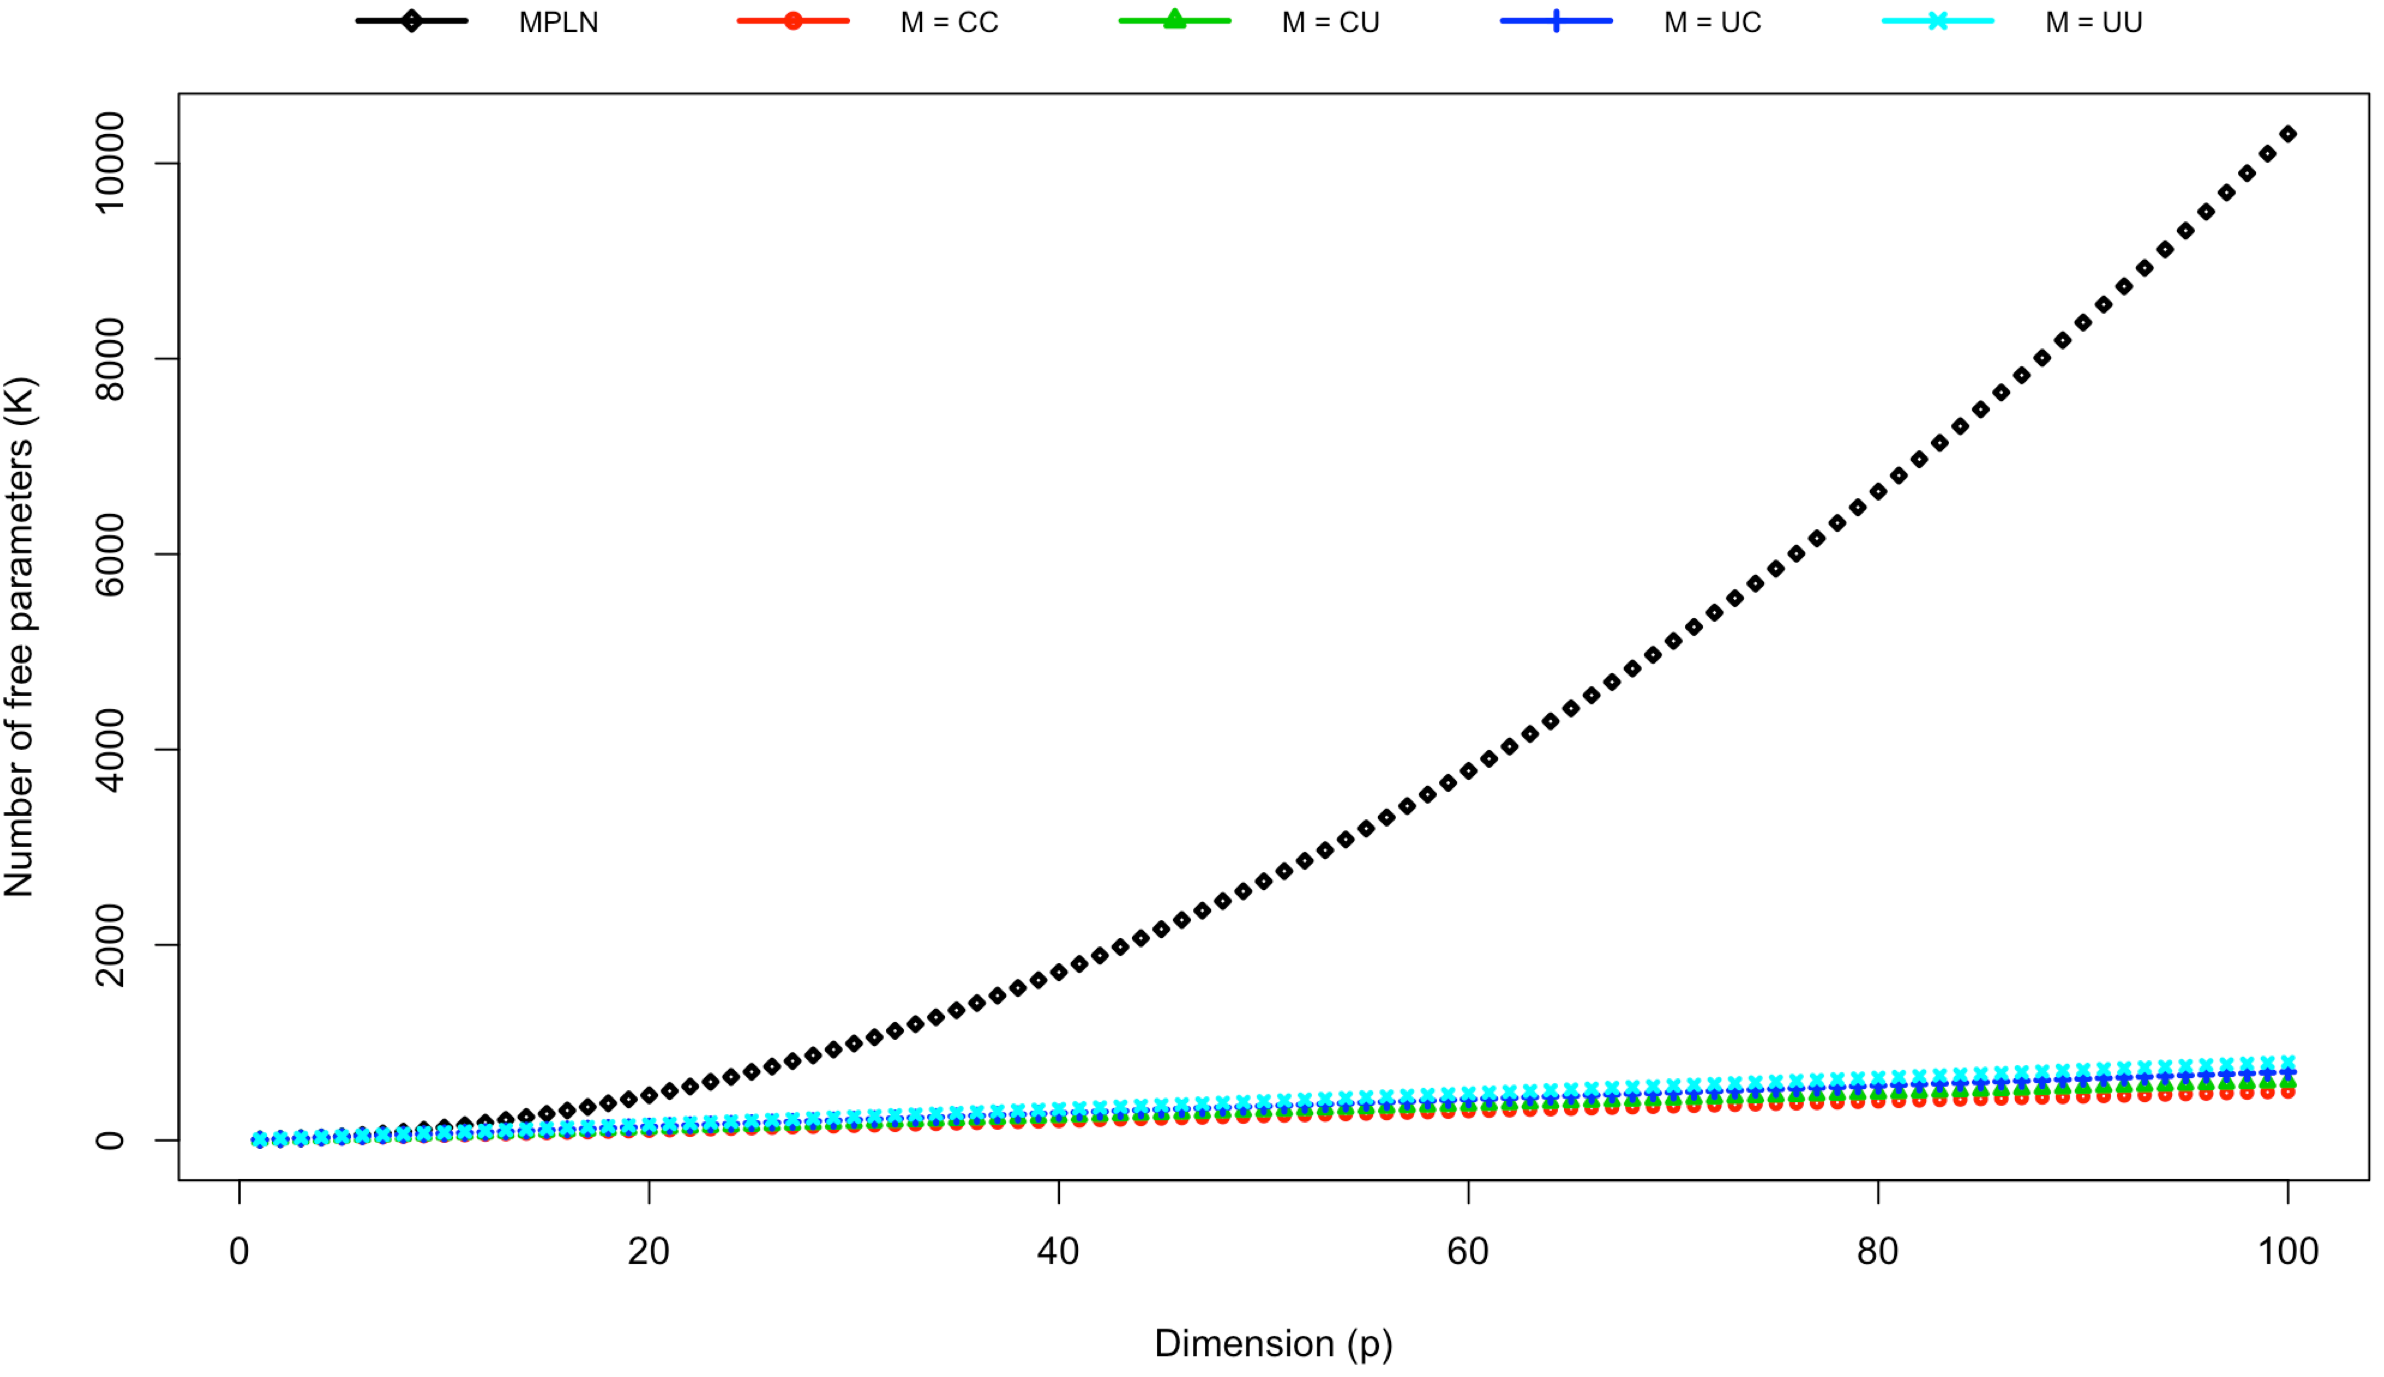
\includegraphics[width=0.84\textwidth]{Chap4_Numb_fparameters_d=1-100,q=2,G=2.png}
\caption{Scatter plot illustrating how the number of free parameters $K$ grows with data dimensionality $p$ for the mixtures of MPLN model and the four members of the PMPLNFA family (M = CC, CU, UC, UU). Here $G = 2, q = 2,$ and $p = 1:100$.} 
\label{freepara1_FAMPLN}
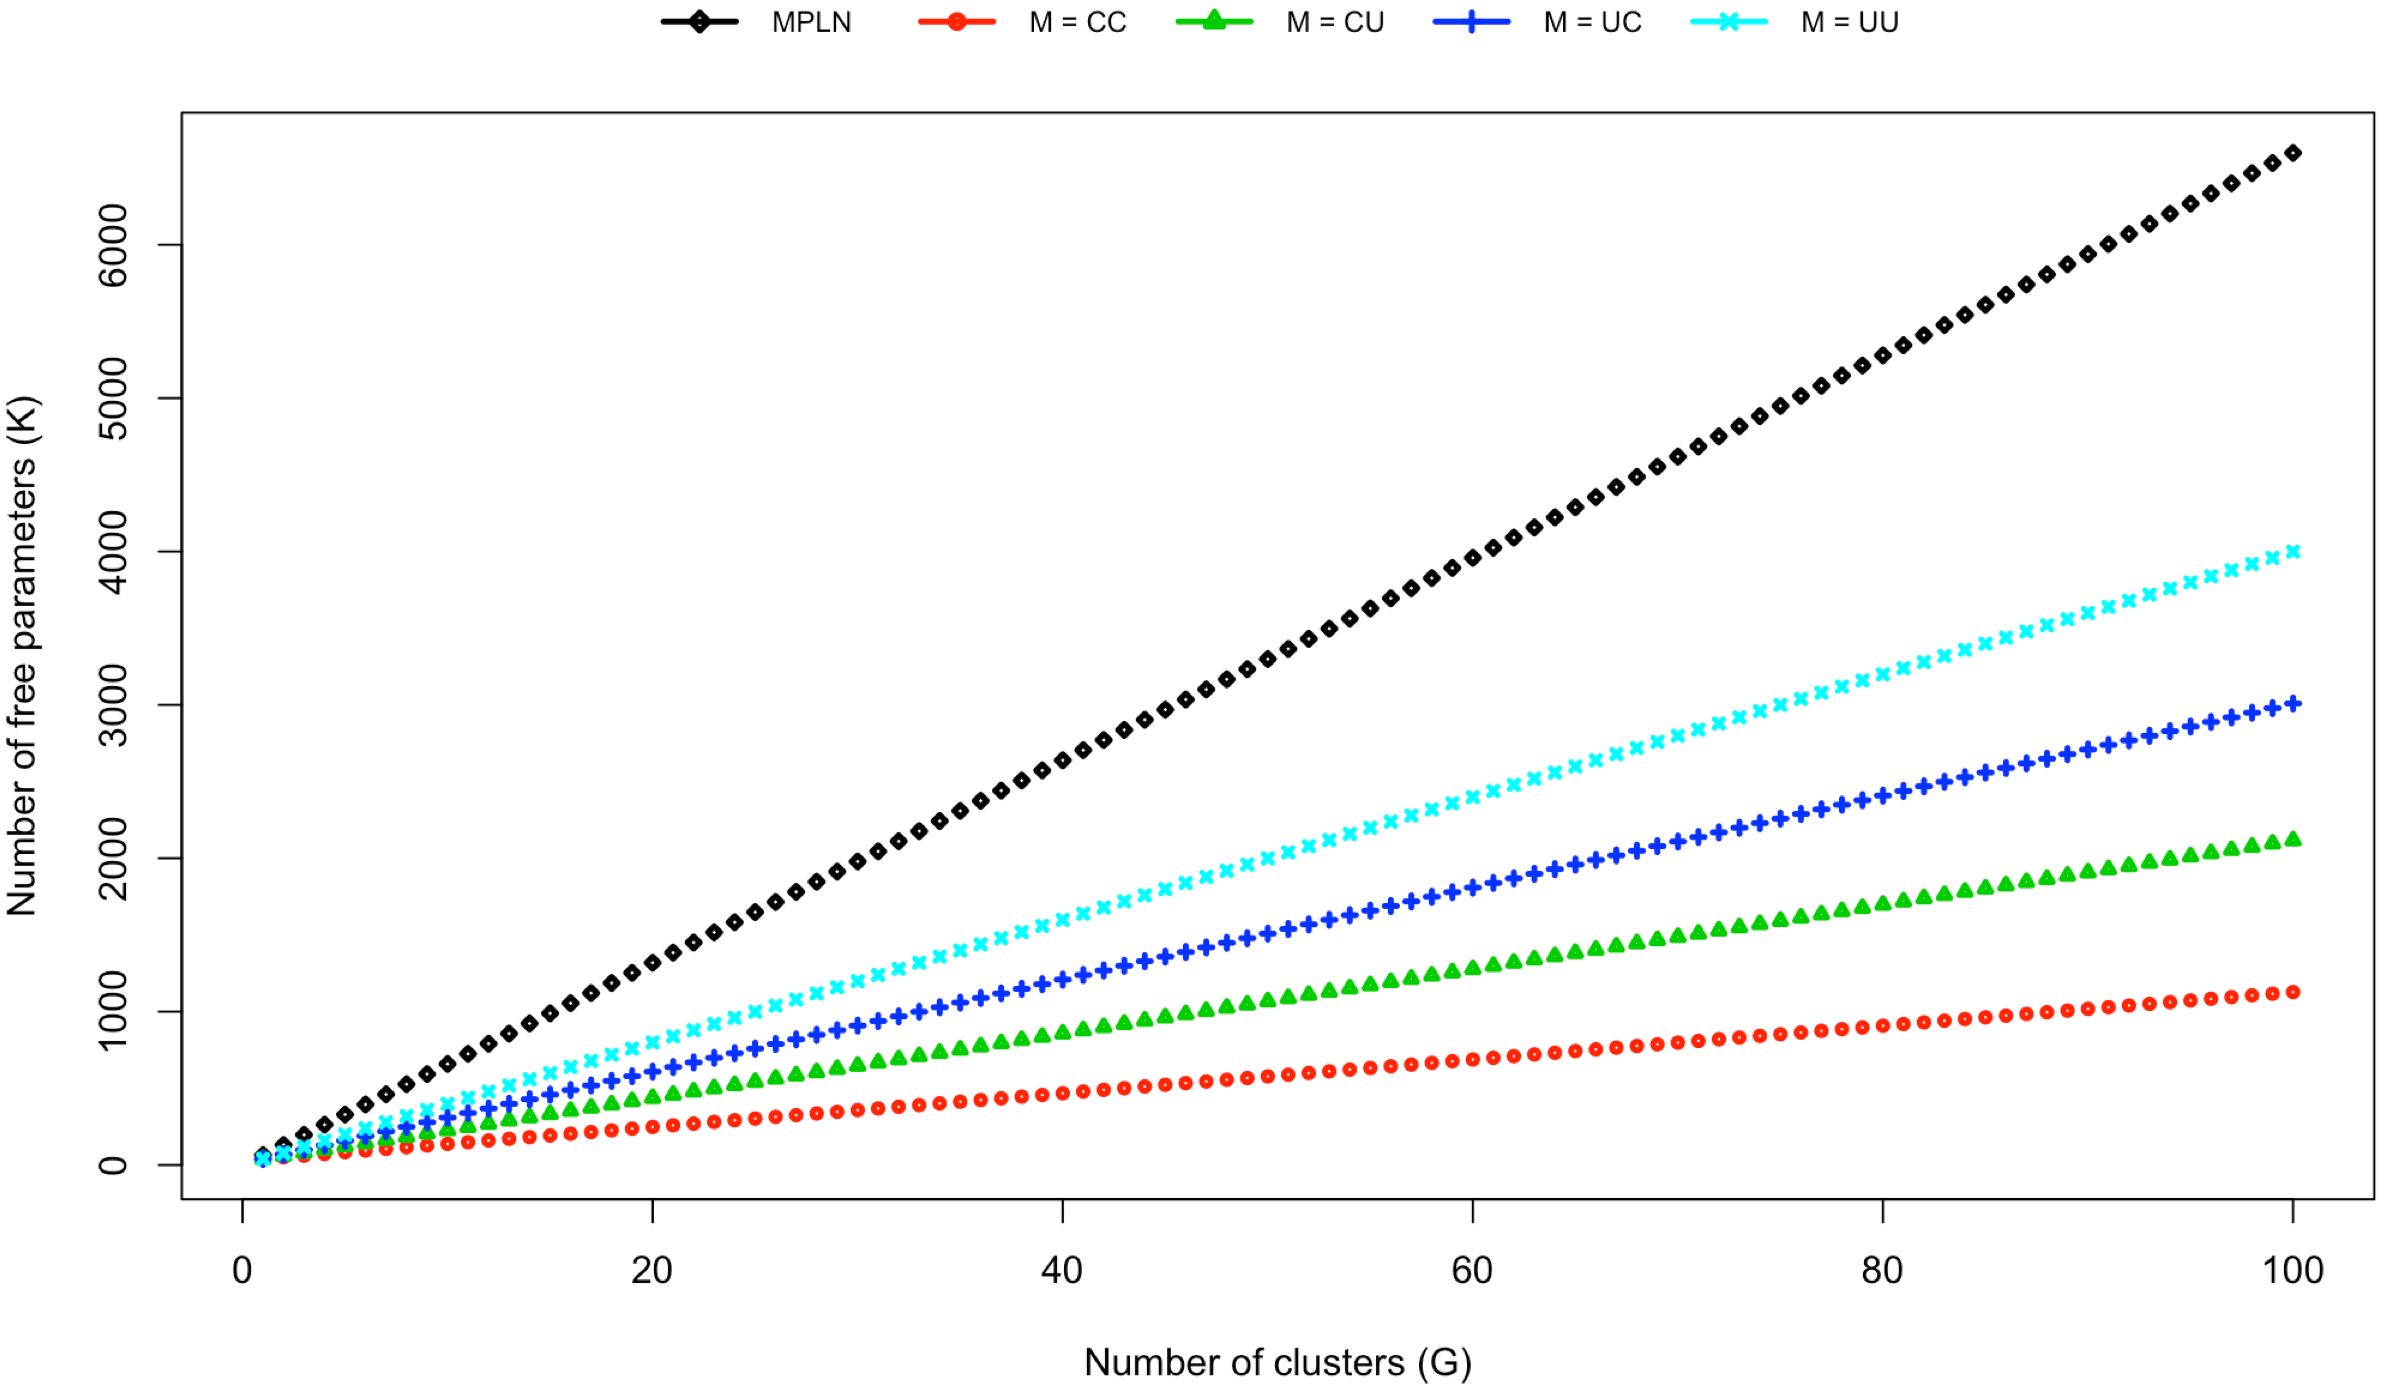
\includegraphics[width=0.84\textwidth]{Chap4_Numb_fparameters_d=10,q=2,G=1-100.png}
\caption{Scatter plot illustrating how the number of free parameters $K$ grows with the number of clusters $G$ for the mixtures of MPLN model and the four members of the PMPLNFA family. Here $G = 1:100, q = 2,$ and $p = 10$.} 
\label{freepara2_FAMPLN}
\end{figure*}

\subsection{Convergence}
Convergence of MCMC-AECM algorithm is determined following the criteria outlined by \citet{Silva2017}. To determine whether the MCMC chains have converged to the posterior distribution, the \textit{potential scale reduction factor} \citep{gelman1992} and the \textit{effective number of samples} \citep{gelman2013} is used. To check if the likelihood has reached its maximum, the Heidelberger and Welch's convergence diagnostic \citep{heidelberger1983} is used.

\subsection{Initialization}
Initialization of $\boldsymbol{\mu}_g$ and $\boldsymbol{S}_g$ is done following the criteria outlined by \citet{Silva2017}. The matrices $\boldsymbol{\Lambda}_g$  and $\boldsymbol{\Psi}_g$ are initialized following \citet{mcnicholas2008} using the eigen-decomposition of $\hat{\boldsymbol{S}}_g^{(0)}$ as follows. The initial values of the $j$th column of $\vecLambda_g$ are set as $\gamma_{j}^{(0)} = \sqrt{d_j}\rho_{ij}$, where $d_j$ is the $j$th largest eigenvalue of $\hat{\boldsymbol{S}}_g^{(0)}$ and $\rho_{ij}$ is the $i$th eigenvector corresponding to the $j$th largest eigenvalue of $\hat{\boldsymbol{S}}_g^{(0)}$ for $i \in \{1, \ldots, p\}$ and $j \in \{1, \ldots, q\}$. The $\matPsi_g$ is then initialized as $\hat{\matPsi}_g^{(0)} = \text{diag}(\hat{\boldsymbol{S}}_g^{(0)}-\hat{\vecLambda}_g^{(0)}\hat{\vecLambda}_g^{(0)^{\prime}})$. For initialization of $\hat{z}_{ig}$, two algorithms are provided: $k$-means and random. For $k$-means initialization, $k$-means clustering is performed on the dataset and the resulting cluster memberships are used for the initialization of $\hat{z}_{ig}$. For random initialization, random values are chosen for $\hat{z}_{ig} \in [0,1]$ such that $\sum_{i=1}^n z_{ig} = 1$ for all $i$. If multiple initialization runs are considered, the $\hat{z}_{ig}$ values corresponding to the run with the highest log-likelihood value are used for downstream analysis.

\subsection{Parallel Implementation}
The algorithm is parallelized using the ${\tt parallel}$ package \citep{r2014} and ${\tt foreach}$ package \citep{foreach2015}, to run each combination of cluster, $G$, latent factor, $q$ and component scale matrix, $M$ in parallel, each one on a different processor. All data analyses were done using the parallelized code. 

\subsection{Model Selection and Performance Assessment}
For this analysis, four model selection criteria are used. These include the Akaike information criterion \citep[$\textsc{AIC}$;][]{akaike1973}, the Bayesian information criterion \citep[$\textsc{BIC}$;][]{schwarz1978}, a variation of the $\textsc{AIC}$ used by \citet{Bozdogan1994} called $\textsc{AIC3}$, and the integrated completed likelihood \citep[$\textsc{ICL}$;][]{biernacki2000}. AIC, BIC, AIC3 and ICL are used to select the best PMPLNFA model in terms of the number of clusters, latent factors, and the structure of the component scale matrices. Performance assessment is done using adjusted Rand index \citep[$\textsc{ARI}$;][]{hubert1985}. 

\subsection{Transcriptome Data Analysis} 
To illustrate the use of PMPLNFA, it was applied to a co-expression analysis of differentially expressed genes identified in the RNA-seq study of cranberry beans (\textit{P. vulgaris}) by \citet{freixascoutin2017}. The study was conducted to evaluate if the changes in the seed coat transcriptome were associated with proanthocyanidin levels as a function of seed development. For this purpose, RNA-seq was used to monitor the transcriptional dynamics in the seed coats of darkening and non-darkening cranberry beans at three developmental stages: early, intermediate and mature. The data are available on the National Center for Biotechnology Information (NCBI) Sequence Read Archive (SRA) under the BioProject PRJNA380220.

The study identified $1336$ differentially expressed genes, which were used for clustering. The raw read counts for genes were obtained from Binary Alignment/Map files using samtools \citep{li2009} and HTSeq \citep{anders2015}. The median value from the $3$ replicates per each developmental stage was used. The genes were clustered for a range of $G = 1, \ldots , 10$ using $k$-means initialization with $3$ runs. To identify if co-expressed genes are implicated in similar biological processes or pathways, a gene ontology (GO) enrichment analysis was performed on the gene clusters using the Singular Enrichment Analysis tool available on AgriGO \citep{du2010}. A significance level of 5\% was used with Fisher statistical testing and Yekutieli multi-test adjustment.

\subsection{Simulation Study}
Simulation studies were conducted to illustrate the ability to recover the true underlying parameters by the PMPLNFA. The count range in all simulated datasets represented count range and library sizes observed in RNA-seq data. Two dimensionality sizes were considered, $p = 6$ and $p = 10$, each with $q = 2$ latent factors for $G = 2$ clusters with $n =  500$ and $\pi_1 = 0.6$. For $p = 6$, data was generated from all the models with covariance structure $ M = \text{CC, CU, UC and UU}$. For $p = 10$, the covariance structure was set to be $M = \text{CC and CU}$. The last simulation setting had $p = 6$, $q = 3$, $G = 1$ and  $M = \text{CC}$. For each of the settings (see Table~\ref{settings_simstudy}), two datasets were generated. Each dataset was run for a clustering range of $G = 1,\ldots, 3$, a latent factor range of $q = 1,\ldots, 3$ and for all four component scale matrices listed in Table~\ref{nomenclature}. All data analyses were performed using $k$-means initialization with $3$ runs.

\begin{table}[h!]
\centering
\caption{Various settings used in the simulation study for PMPLNFA.}
\label{settings_simstudy}
\resizebox{\textwidth}{!}{%
\begin{tabular}{lllll}
\hline
Setting & Cluster, $G$ & Latent factor, $q$ & Component scale matrix, $M$ & Dimensions \\ \hline
1         & 2 & 2 & CC      & 500 x 6         \\
2        & 2 & 2 & CU      & 500 x 6         \\
3        & 2 & 2 & UC      & 500 x 6         \\
4        & 2 & 2 & UU      & 500 x 6        \\
5        & 2 & 2 & CC      & 500 x 10        \\
6        & 2 & 2 & CU      & 500 x 10       \\
7        & 1 & 3 & CC      & 500 x 6         \\ \hline
\end{tabular}}
\end{table}

For both real and simulation data analyses, the normalization factors representing library size estimate for samples were obtained using the trimmed mean of M values from ${\tt calcNormFactors}$ function of ${\tt edgeR}$ package \citep{robinson2010, mccarthy2012}. All data analyses were performed on a MacBook Pro with $3.1$ GHz quad-core Intel Core i7 processor and $16$ GB RAM, and the Joyce high performance computing cluster at the McMaster University, Hamilton, ON, Canada. The Joyce system is an Intel(R) Xeon(R) CPU E5-4627 v2 with $32$ cores, $3.3$ GHz and 256 GB RAM.

\subsection{Software availability}
The source code is made available at \texttt{https://github.com/anjalisilva/mixMPLNFA} and is released under the open source MIT license.

\section{Results}
\subsection{Transcriptome Data Analysis} 

\begin{figure*}[]
\centering
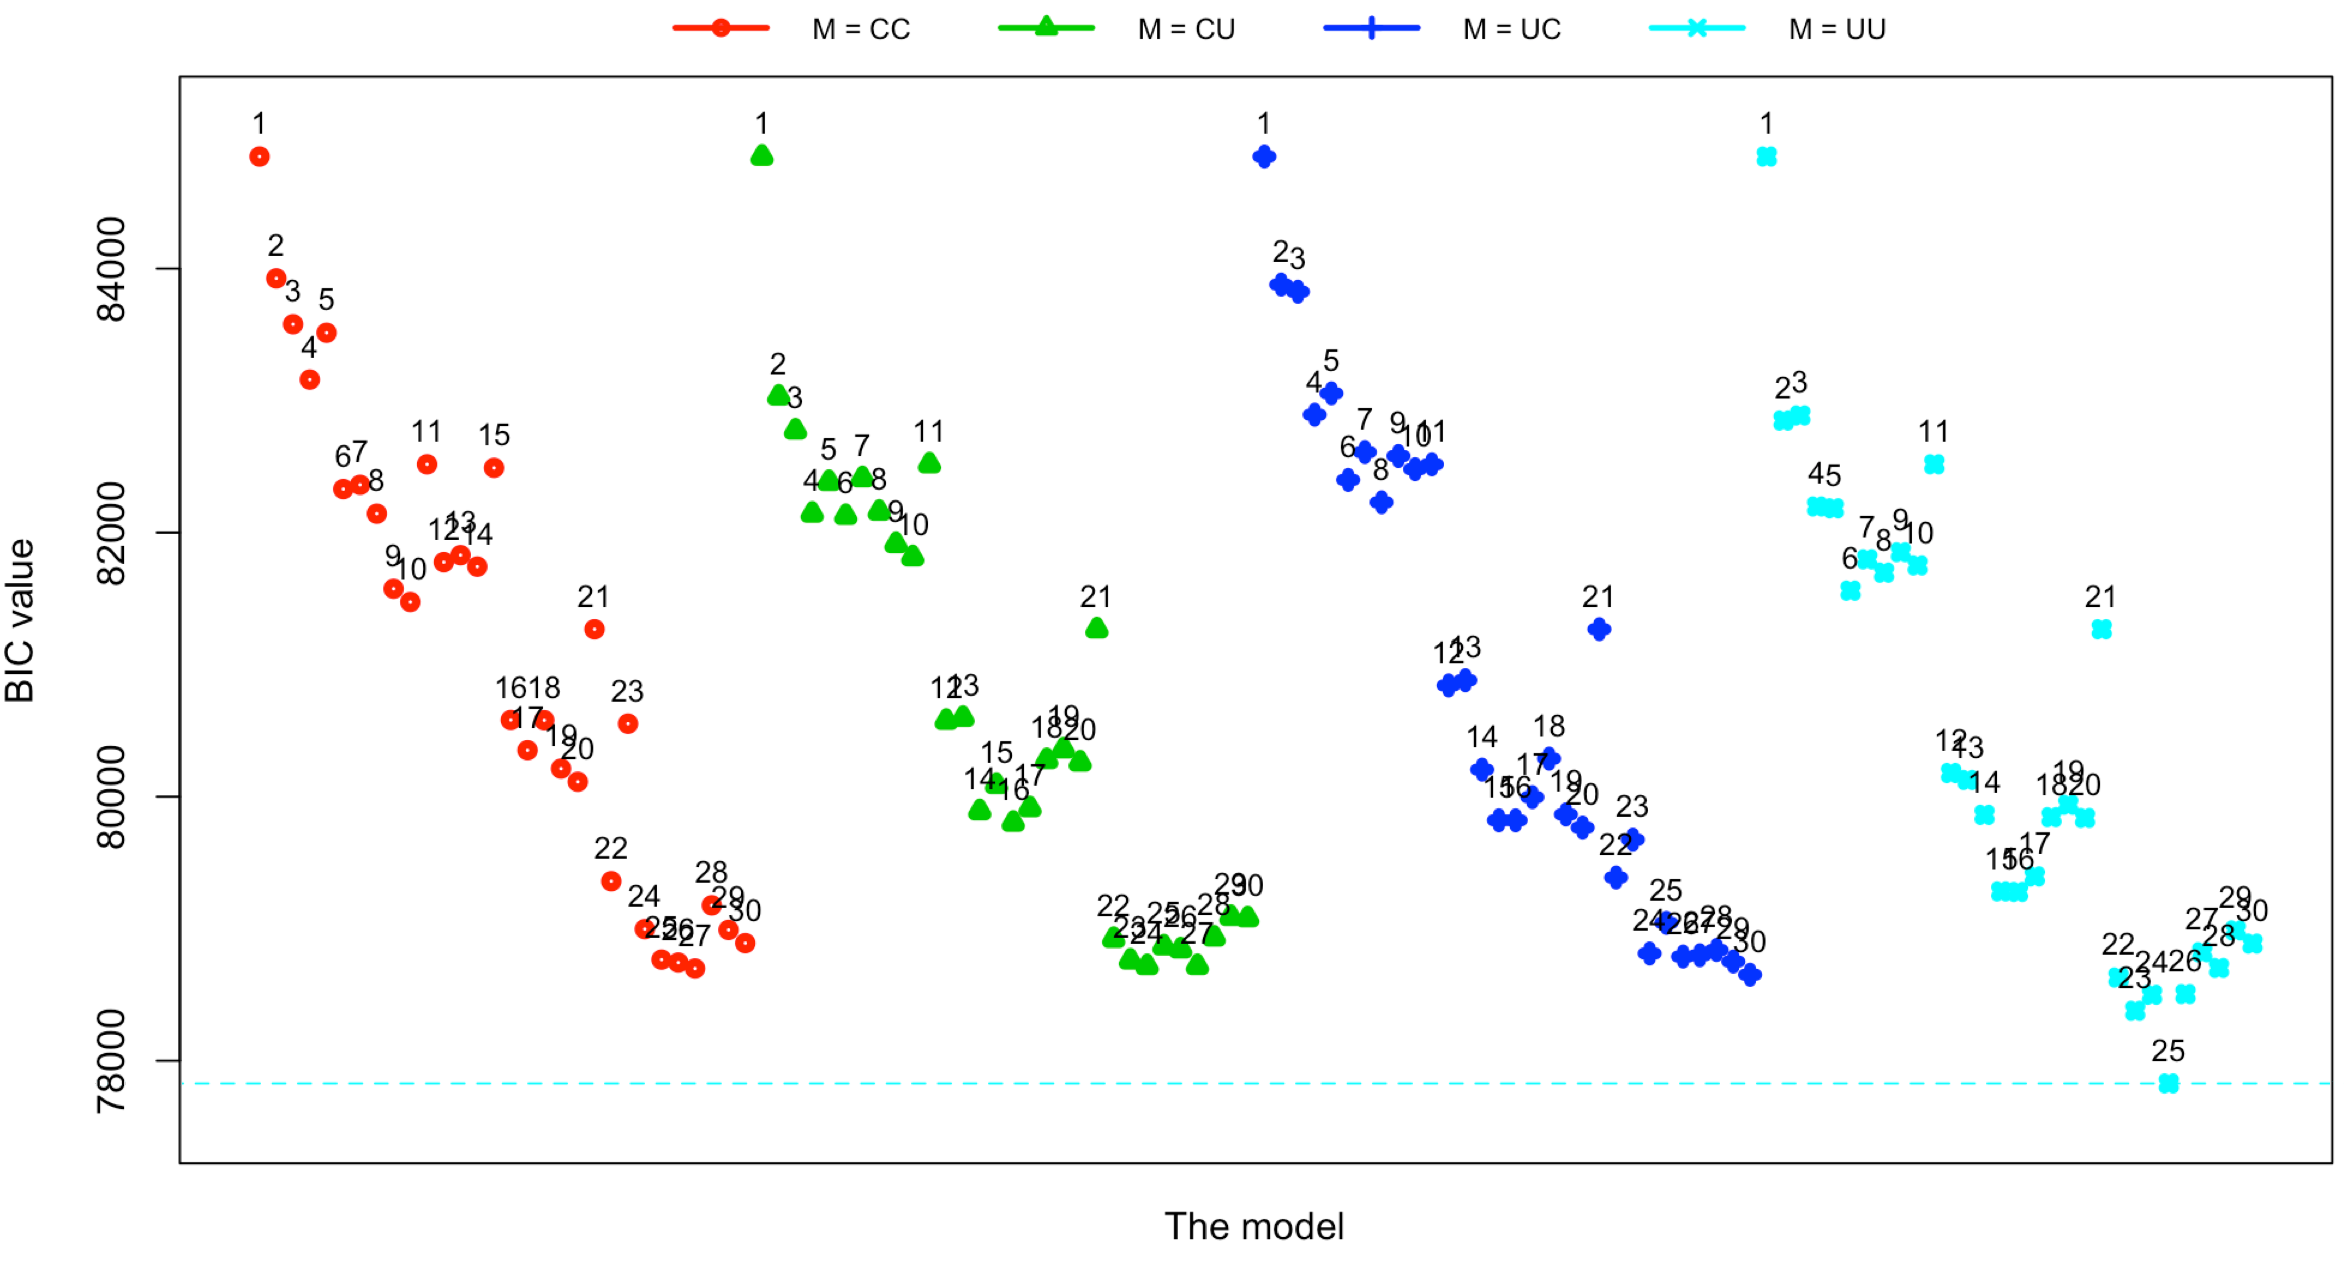
\includegraphics[width=0.85\textwidth]{Chap4_FA_Bozzo_modelselection.png}
\caption{Plot of BIC value versus the model for the cranberry bean RNA-seq data. Numbers denote the corresponding model and the color denotes the component scale matrix $M$. Model~1 is $(G=1,q=1)$, model~2 is $(G=2,q=1)$, model~3 is $(G=3,q=1)$, $\ldots.$  The dotted line indicates the model selected by BIC, which is $G=5,q=3,M=\text{UU}$.} 
\label{valuevscluster_FA}
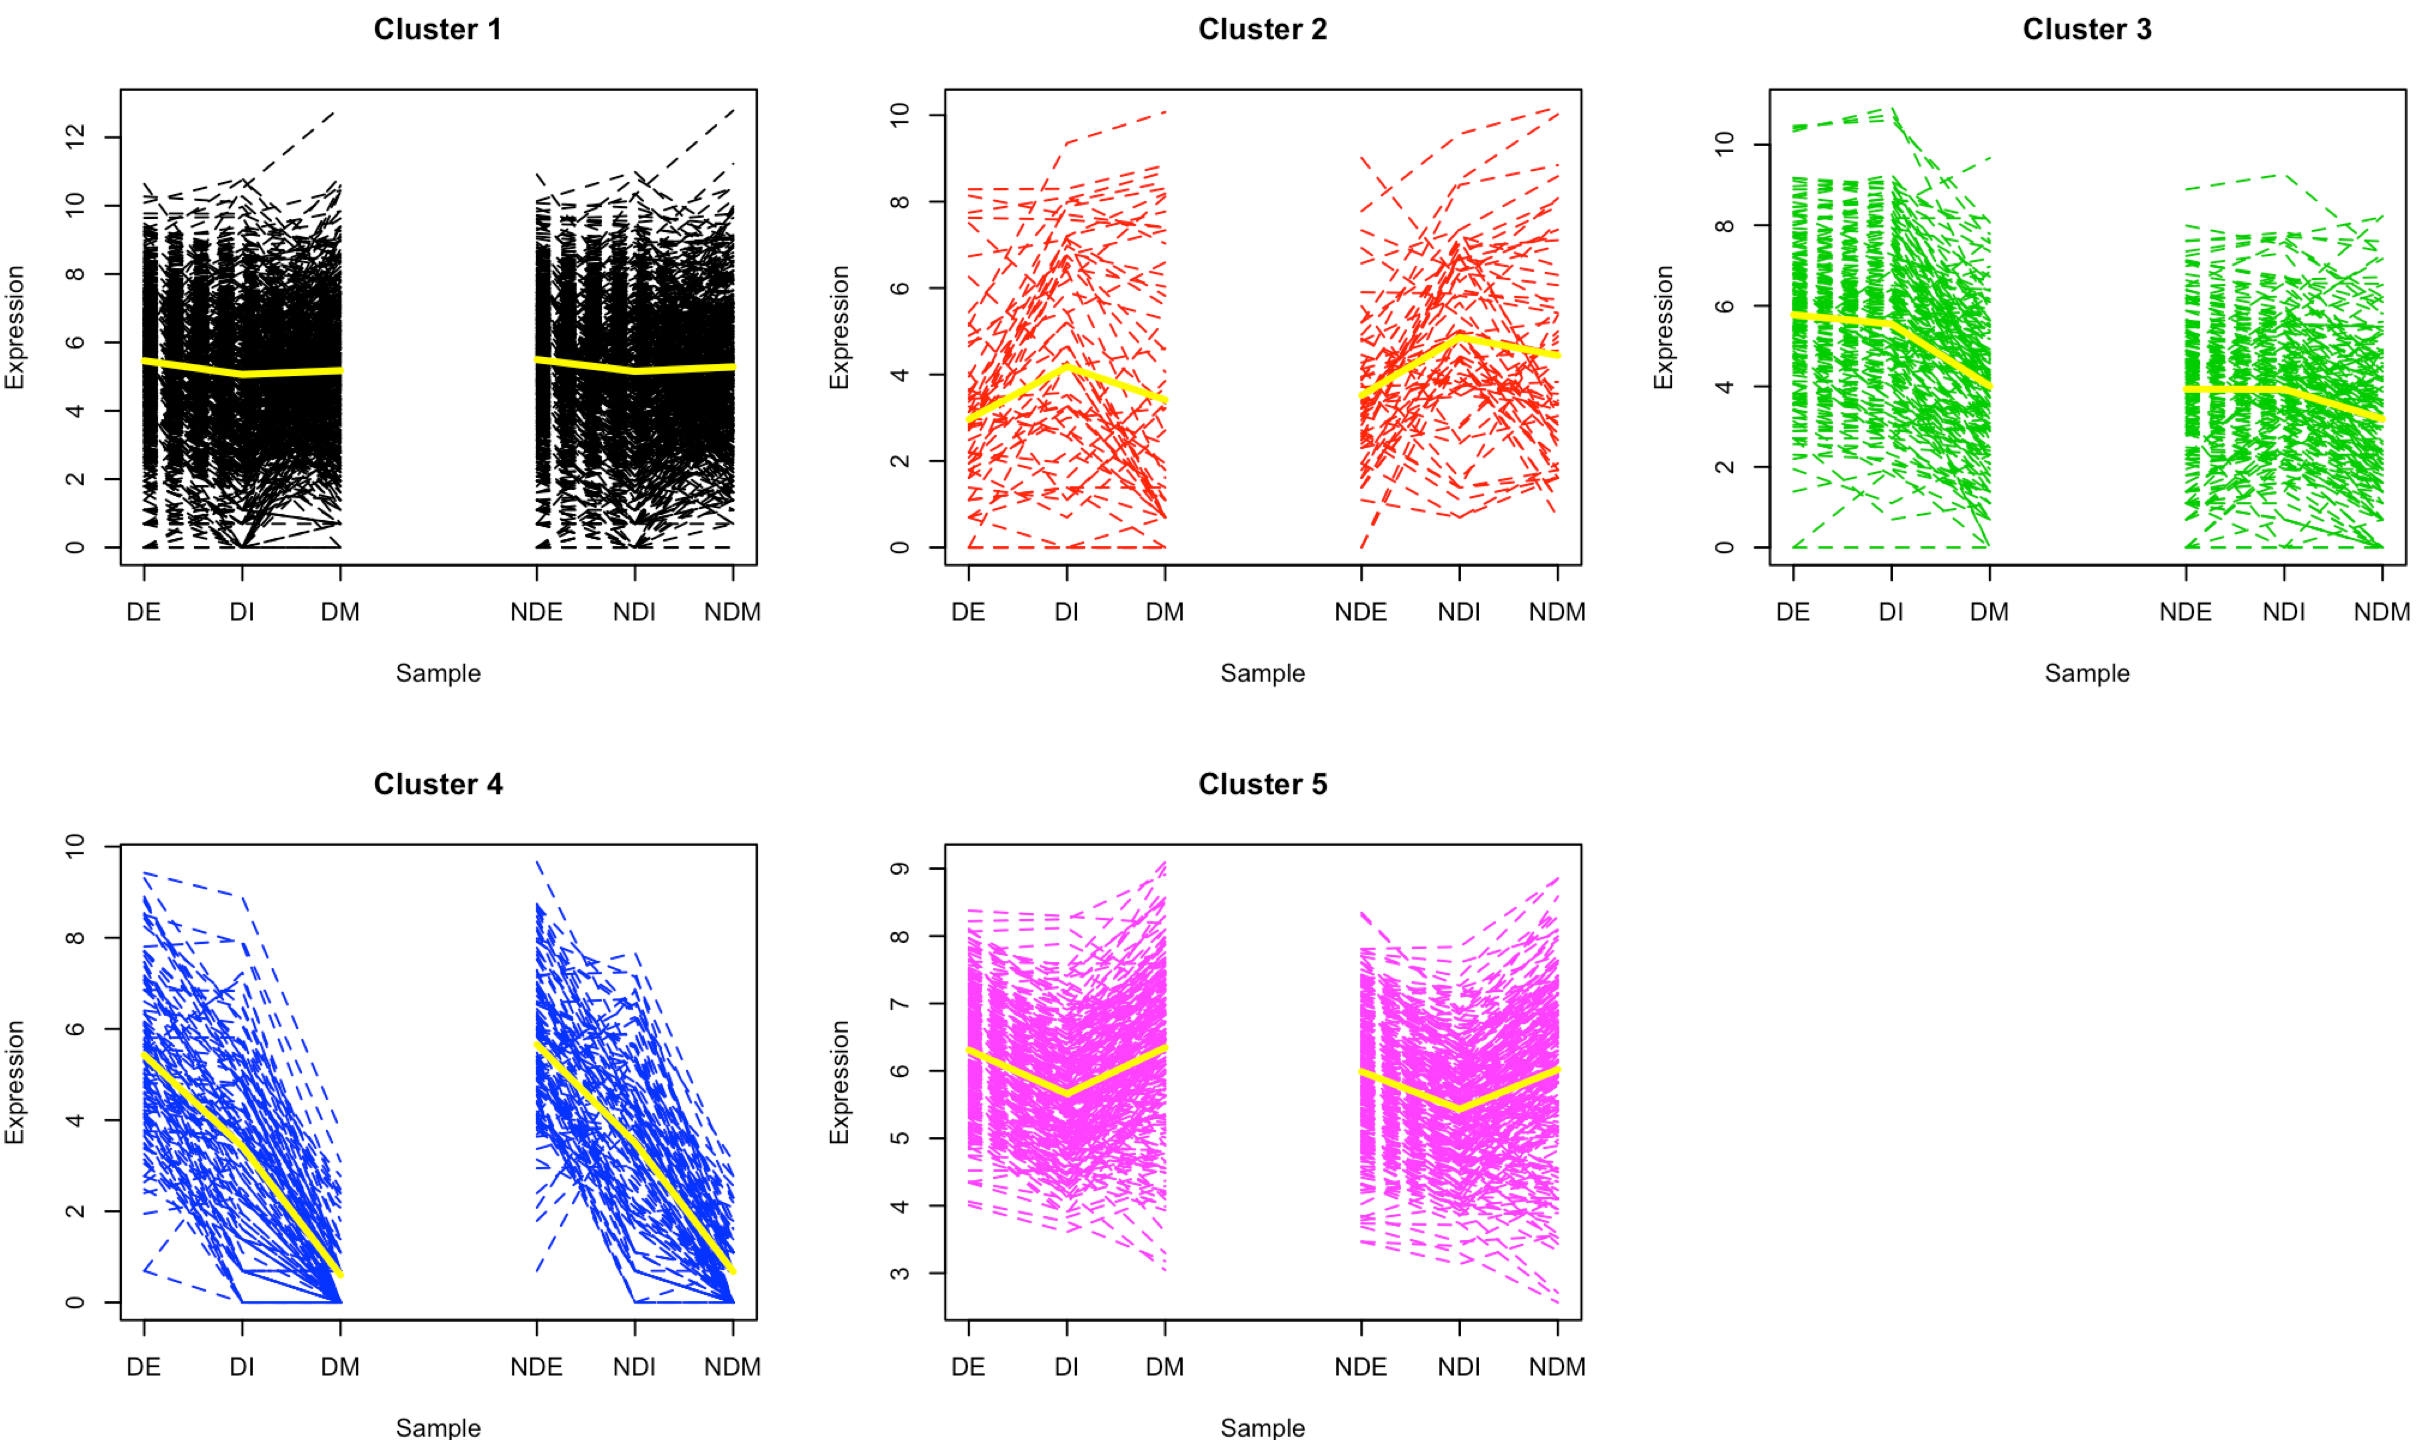
\includegraphics[width=0.85\textwidth]{Chap4_FAMPLN_bozzo_trends2.png}
\caption{The expression patterns for the five clusters in the $G = 5, q = 3$ and $M = \text{UU}$ model selected by all information criteria for the cranberry bean RNA-seq data. The expression is in log-transformed counts. The yellow line represents the mean expression level for each cluster. The samples are DE:  darkening early, DI: darkening intermediate, DM: darkening mature, NDE: non-darkening early, NDI: non-darkening intermediate and NDM: non-darkening mature.}
\label{paper2_bozzo_trends}
\end{figure*}

All information criteria selected a model with $G = 5, q = 3$ and $M = \text{UU}$ for the cranberry bean RNA-seq study. The clustering results via BIC for transcriptome data are summarized on Figure~\ref{valuevscluster_FA}. The expression patterns among the different clusters for this model are provided in Figure~\ref{paper2_bozzo_trends}. The compositions of genes in Clusters~1 through~5 were as follows:~722, 59, 180, 111 and 264. Cluster~1 genes were expressed roughly constantly across all samples. The GO enrichment analysis identified genes belonging to oxidation reduction, dehydrogenase activity, binding and electron carrier activity. Cluster~2 genes showed variable expression and belonged to pathogenesis and multi-organism process. 

Cluster~3 genes showed higher expression in early and intermediate developmental stages relative to mature developmental stage, across both the darkening and non-darkening varieties. These genes belonged to lipid/ fatty acid biosynthesis, lipid/ fatty acid metabolic process, synthase activity and transferase activity. Cluster~4 expression patterns revealed higher expression in early developmental stage and gradual decrease during intermediate followed by mature developmental stage. GO enrichment analysis identified binding, hydrolase activity, oxidoreductase activity and catalytic activity. Finally, Cluster~5 expression patterns revealed lower expression in intermediate developmental stage relative to other developmental stages, regardless of the variety. These genes belonged to hydrolase activity, ATPase activity, pyrophosphatase activity, nucleoside-triphosphatase activity and aromatic amino acid family metabolic process. 

Due to the similarities in Clusters~1 and~4, with respect to GO enrichment terms, these clusters were further analyzed. Although both clusters were enriched for binding, Cluster~1 was enriched for iron ion binding (GO:0005506), heme binding (GO:0020037) and tetrapyrrole binding (GO:0046906). Conversely, Cluster~4 was enriched for coenzyme binding (GO:0050662) and flavin adenine dinucleotide (FAD)-binding (GO:0050660). In terms of oxidation reduction, Cluster~1 was enriched for oxidoreductase activity, acting on paired donors, with incorporation or reduction of molecular oxygen (GO:0016705). However, Cluster~4 was enriched for oxidoreductase activity, acting on the CH-OH group of donors, nicotinamide adenine dinucleotide (NAD) or nicotinamide adenine dinucleotide phosphate (NADP) as acceptor (GO:0016616) and oxidoreductase activity, acting on CH-OH group of donors (GO:0016614). Overall, the results obtained from GO annotations suggest distinct themes among the five clusters. 

\subsection{Simulation Study}
The clustering results obtained using different model selection criteria and corresponding average ARI values are summarized in Table~\ref{table_g2modelselection}. The model selection criteria gave comparable results in terms of the number of clusters and the number of latent factors, however, occasionally AIC and AIC3 failed to select the correct number of clusters. In such situations, AIC and AIC3 selected a higher number of clusters. Across all settings, the ARI values were equal to or very close to one, indicating that the algorithm is able to assign observations to the proper clusters, i.e., the clusters that were originally used to generate the simulation datasets. In terms of selecting the component scale matrix, both AIC and AIC3 selected the incorrect model for some settings. In these situations, the unconstrained loading matrix or the unconstrained error variance was selected. Overall, the simulation experiments illustrate that the proposed algorithm is able to recover proper clusters, latent factors and the component scale matrix for PMPLNFA.

\begin{table*}[h!]
\centering
\caption{Model selection results of the clusters (average ARI, standard deviation), latent factors and component scale matrices for each simulation setting using different model selection criteria.}
%\vspace{3mm}
\label{table_g2modelselection}
\resizebox{\textwidth}{!}{%
\begin{tabular}{@{\extracolsep{-9pt}}ccccccccccccccccccc@{}}
\hline
 && \multicolumn{4}{c}{Cluster, $G$} & \hspace{5mm }& \hspace{5mm } & \multicolumn{4}{c}{Latent factor, $q$} &\hspace{5mm } & \hspace{5mm }& \multicolumn{4}{c}{Component scale matrix,  $M$} \\
\cline{3-6} \cline{9-12} \cline{15-18} 
Setting   && BIC        & ICL         & AIC             & AIC3           & \hspace{5mm }& \hspace{5mm }& BIC & ICL & AIC & AIC3 &\hspace{1mm } & & BIC & ICL & AIC & AIC3 \\ \hline
1 && 2 & 2  & 2       & 2       & \hspace{5mm }& \hspace{5mm }& 2     & 2    & 2      & 2      &\hspace{0.5 mm }& & CC & CC   & UC       & CC \\
  &&  (0.99, 0.01) & (0.99, 0.01) & (0.99, 0.01) & (0.99, 0.01)      & \hspace{5mm }& \hspace{5mm }&      &       &         &       &\hspace{0.5 mm } & &   &    &       &  \\
2 && 2 & 2 & 2        & 2       & \hspace{5mm }& \hspace{5mm }& 2     & 2    & 2      & 2      & \hspace{0.5 mm }& & CU & CU   & CU       & CU  \\
 &&  (1.00, 0.00) &  (1.00, 0.00) &  (1.00, 0.00)       & (1.00, 0.00)       & \hspace{5mm }& \hspace{5mm }&      &     &       &       & \hspace{0.5 mm }& & &   &      &  \\
3 && 2  & 2  & 2        & 2       & \hspace{5mm }& \hspace{5mm }& 2     & 2    & 2      & 2      &\hspace{0.5 mm }& & UC & UC   & UU       & UU \\
 && (1.00, 0.00) & (1.00, 0.00) & (1.00, 0.00)       & (1.00, 0.00)       & \hspace{5mm }& \hspace{5mm }&      &    &      &       &\hspace{0.5 mm }& &  &  &       &  \\
4 && 2  & 2  & 2       & 2       & \hspace{5mm }& \hspace{5mm }& 2     & 2    & 2      & 2      & \hspace{0.5 mm }& & UU & UU   & UU       & UU \\
 && (1.00, 0.00) & (1.00, 0.00) & (1.00, 0.00)       & (1.00, 0.00)       & \hspace{5mm }& \hspace{5mm }&      &     &       &       & \hspace{0.5 mm }& & &    &        &  \\
5 && 2  & 2  & 2--3  & 2--3  & \hspace{5mm }& \hspace{5mm }& 2     & 2    & 2      & 2     & \hspace{0.5 mm }& & CC & CC    & CC/CU & CC/CU \\
 &&  (1.00, 0.00) &  (1.00, 0.00) & (0.99, 0.01) & (0.99, 0.01) & \hspace{5mm }& \hspace{5mm }&      &     &      &     & \hspace{0.5 mm }& & &   &  &  \\
6 && 2  & 2 & 2       & 2       & \hspace{5mm }& \hspace{5mm }& 2     & 2    & 2      & 2     & \hspace{0.5 mm }& & CU & CU    & CU        & CU \\ 
 &&  (1.00, 0.00) &  (1.00, 0.00) & (1.00, 0.00)       & (1.00, 0.00)       & \hspace{5mm }& \hspace{5mm }&      &     &       &      & \hspace{0.5 mm }& &  &     &         &  \\ 
7 && 1  & 1  & 1        & 1         & \hspace{5mm }& \hspace{5mm }& 3     & 3    & 3       & 3     & \hspace{1mm }& & CC & CC    & CC        & CC \\ 
 && (1.00, 0.00)  & (1.00, 0.00)  & (1.00, 0.00)        & (1.00, 0.00)         & \hspace{5mm }& \hspace{5mm }&      &    &       &      & \hspace{1mm }& &  &     &         &  \\  
 
\hline
\end{tabular}}
\end{table*}

\section{Discussion}\label{sec:discussion}
A mixture of factor analyzers model for MPLN distribution as well as a family of mixture models based thereon is introduced. This is the first use of a mixture of MPLN factor analyzer distributions within the literature. To our knowledge, this is also the first use of a mixture of discrete factor analyzers within the literature. The proposed models are well-suited to high-dimensional applications as the number of scale parameters is linear in data dimensionality for all four models, as opposed to in traditional MPLN, where the parameters grow quadratically. The PMPLNFA family of models can be easily extended to consider an isotropic noise. Further, a MPLN factor analysis model can be obtained as a special case of the mixture of PMPLNFA, i.e., with $G = 1$. Extensions applicable to factor analyzers model, such as the mixture of common factor analyzers \citep{Baek2010} can be applied to the PMPLNFA family in future. A mixture of common factor analyzers is a restrictive form of the mixture of factor analyzers model and can be useful when the number of clusters and dimensionality are very large. 

\subsection*{Acknowledgments}
{\small This research was supported by the Ontario Graduate Fellowship (Silva), Arthur Richmond Memorial Scholarship (Silva), and the Canada Natural Sciences and Engineering Research Council grant 400920-2013 (Subedi).}

%\bibliographystyle{chicago}
%\bibliography{bibofA}

{\small
\begin{thebibliography}{}
\bibitem[\protect\citeauthoryear{Aitchison and Ho}{Aitchison and Ho}{1989}]{aitchison1989}
Aitchison, J. and C.~H. Ho (1989).
\newblock The multivariate {P}oisson-log normal distribution.
\newblock {\em Biometrika\/}~{\em 76\/}(4), 643--653.

\bibitem[\protect\citeauthoryear{Akaike}{Akaike}{1973}]{akaike1973}
Akaike, H. (1973).
\newblock Information theory and an extension of the maximum likelihood
  principle.
\newblock In {\em Second International Symposium on Information Theory}, pp.\
  267--281. Springer Verlag.
  
\bibitem[\protect\citeauthoryear{Anders, Pyl, and Huber}{Anders
  et~al.}{2015}]{anders2015}
Anders, S., P.~T. Pyl, and W.~Huber (2015).
\newblock {HTSeq-a Python framework to work with high-throughput sequencing
  data}.
\newblock {\em Bioinformatics\/}~{\em 31\/}(2), 166--169.

\bibitem[\protect\citeauthoryear{Annis, Miller, and Palmeri}{Annis
  et~al.}{2016}]{stan}
Annis, J., B.~J. Miller, and T.~J. Palmeri (2016).
\newblock {Bayesian inference with Stan: A tutorial on adding custom
  distributions}.
\newblock {\em Behavior Research Methods\/}~{\em 49}, 1--24.

\bibitem[\protect\citeauthoryear{Baek, McLachlan, and Flack}{Baek
  et~al.}{2010}]{Baek2010}
Baek, J., G.~J.~McLachlan, and L.~K. Flack (2010).
\newblock Mixtures of factor analyzers with common factor loadings: applications to the clustering and visualization of high-dimensional data.
\newblock {\em IEEE Trans Pattern Anal Mach Intelligence\/}~{\em 32\/}, 1298--1309.

\bibitem[\protect\citeauthoryear{Biernacki, Celeux, and Govaert}{Biernacki
  et~al.}{2000}]{biernacki2000}
Biernacki, C., G.~Celeux, and G.~Govaert (2000).
\newblock Assessing a mixture model for clustering with the integrated
  classification likelihood.
\newblock {\em IEEE Transactions on Pattern Analysis and Machine
  Intelligence\/}~{\em 22\/}(7), 719--725.
 
\bibitem[\protect\citeauthoryear{Bouveyron and Brunet}{Bouveyron and Brunet}{2014}]{bouveyron2012}
Bouveyron, C.~J. and C. Brunet (2014).
\newblock Model-based clustering of high-dimensional data: A review.
\newblock {\em Computational Statistics and Data Analysis\/}~{\em 71}, 52--78.

\bibitem[\protect\citeauthoryear{Bozdogan}{Bozdogan}{1994}]{Bozdogan1994}
Bozdogan, H. (1994).
\newblock Mixture-model cluster analysis using model selection criteria and a
  new informational measure of complexity.
\newblock In {\em Proceedings of the First US/Japan Conference on the Frontiers
  of Statistical Modeling: An Informational Approach: Volume 2 Multivariate
  Statistical Modeling}, pp.\ 69--113. Dordrecht: Springer Netherlands.

\bibitem[\protect\citeauthoryear{Du, Zhou, Ling, Zhang, and Su}{Du
  et~al.}{2010}]{du2010}
Du, Z., X.~Zhou, Y.~Ling, Z.~Zhang, and Z.~Su (2010).
\newblock {agriGO: a GO analysis toolkit for the agricultural community}.
\newblock {\em Nucleic Acids Research\/}~{\em 38}, W64--W70.
  
\bibitem[\protect\citeauthoryear{Freixas-Coutin, Munholland, Silva, Subedi,
  Lukens, Crosby, Pauls, and Bozzo}{Freixas-Coutin
  et~al.}{2017}]{freixascoutin2017}
Freixas-Coutin, J.~A., S.~Munholland, A.~Silva, S.~Subedi, L.~Lukens, W.~L.
  Crosby, K.~P. Pauls, and G.~G. Bozzo (2017).
\newblock Proanthocyanidin accumulation and transcriptional responses in the
  seed coat of cranberry beans {(\textit{Phaseolus vulgaris} L)} with different
  susceptibility to postharvest darkening.
\newblock {\em BMC Plant Biology\/}~{\em 17\/}(89).

\bibitem[\protect\citeauthoryear{Gelman, Carlin, Stern, Dunson, Vehtari, and
  Rubin}{Gelman et~al.}{2013}]{gelman2013}
Gelman, A., J.~B. Carlin, H.~S. Stern, D.~B. Dunson, A.~Vehtari, and D.~B.
  Rubin (2013).
\newblock {\em Bayesian Data Analysis}.
\newblock Boca Raton, FL: Chapman \& Hall/CRC Press.

\bibitem[\protect\citeauthoryear{Gelman and Rubin}{Gelman and
  Rubin}{1992}]{gelman1992}
Gelman, A. and D.~B. Rubin (1992).
\newblock Inference from iterative simulation using multiple sequences.
\newblock {\em Stat Sci\/}~{\em 7\/}(4), 457--472.

\bibitem[\protect\citeauthoryear{Ghahramani and Hinton}{Ghahramani and Hinton}{1997}]{ghahramani1997}
Ghahramani, Z. and G.~E.~Hinton (1997).
\newblock The {EM} algorithm for mixtures of factor analyzers.
\newblock Technical Report  CRG-TR-96-1\ University of Toronto.

\bibitem[\protect\citeauthoryear{Heidelberger and Welch}{Heidelberger and
  Welch}{1983}]{heidelberger1983}
Heidelberger, P. and P.~D. Welch (1983).
\newblock Simulation run length control in the presence of an initial
  transient.
\newblock {\em Operations Research\/}~{\em 31\/}(6), 1109--1144.

\bibitem[\protect\citeauthoryear{Hubert and Arabie}{Hubert and
  Arabie}{1985}]{hubert1985}
Hubert, L. and P.~Arabie (1985).
\newblock Comparing partitions.
\newblock {\em Journal of Classification\/}~{\em 2}, 193--218.

\bibitem[\protect\citeauthoryear{Junk-Knievel, Vandenberg, and
  Bett}{Junk-Knievel et~al.}{2008}]{Junk-Knievel2008}
Junk-Knievel, D.~C., A.~Vandenberg, and K.~E. Bett (2008).
\newblock Slow darkening in {pinto bean (\textit{Phaseolus vulgaris} L)} seed
  coats is controlled by a single major gene.
\newblock {\em Crop Science\/}~{\em 48\/}(1), 189--193.

\bibitem[\protect\citeauthoryear{Lawley and Maxwell}{Lawley and Maxwell}{1962}]{lawley1962}
Lawley, D.~N. and A.~E.~Maxwell (1962).
\newblock Factor analysis as a statistical method.
\newblock {\em Journal of the Royal Statistical Society: Series~D\/}~{\em 12\/}, 209--229.

\bibitem[\protect\citeauthoryear{Li, Handsaker, Wysoker, Fennell, Ruan, Homer, Marth, Abecasis, Durbin, and Subgroup}{Li et~al.}{2009}]{li2009}
Li, H., B.~Handsaker, A.~Wysoker, T.~Fennell, J.~Ruan, N.~Homer, G.~Marth,
  G.~Abecasis, R.~Durbin, and .~G. P. D.~P. Subgroup (2009).
\newblock {The Sequence alignment/map (SAM) format and SAMtools}.
\newblock {\em Bioinformatics\/}~{\em 25\/}(16), 2078--2079.

\bibitem[\protect\citeauthoryear{McCarthy, Chen, and Smyth}{McCarthy
  et~al.}{2012}]{mccarthy2012}
McCarthy, J.~D., Y.~Chen, and K.~G. Smyth (2012).
\newblock Differential expression analysis of multifactor {RNA-Seq} experiments
  with respect to biological variation.
\newblock {\em Nucleic Acids Research\/}~{\em 40\/}(10), 4288--4297.

\bibitem[\protect\citeauthoryear{McLachlan and Basford}{McLachlan and
  Basford}{1988}]{mclachlanandbasford1998}
McLachlan, G.~J. and K.~E. Basford (1988).
\newblock {\em Mixture Models Inference and Applications to Clustering}.
\newblock New York: Marcel Dekker.

\bibitem[\protect\citeauthoryear{McLachlan and Peel}{McLachlan and
  Peel}{2000}]{mclachlan2000}
McLachlan, G.~J. and D.~Peel (2000).
\newblock {\em {Finite Mixture Models}}.
\newblock New York: Wiley.

\bibitem[\protect\citeauthoryear{McNicholas}{McNicholas}{2016}]{mcnicholas2016}
McNicholas, P.~D. (2016).
\newblock {\em {Mixture Model-based Classification}}.
\newblock Boca Raton: Chapman and Hall/CRC Press.

\bibitem[\protect\citeauthoryear{McNicholas and Murphy}{McNicholas and Murphy}{2010}]{mcnicholas2010}
McNicholas, P.~D. and T.~B.~Murphy (2010).
\newblock Model-based clustering of microarray expression data via latent {G}aussian mixture models.
\newblock {\em Bioinformatics\/}~{\em 26\/}, 2705--2712.

\bibitem[\protect\citeauthoryear{McNicholas and Murphy}{McNicholas and Murphy}{2008}]{mcnicholas2008}
McNicholas, P.~D. and T.~B.~Murphy (2008).
\newblock Parsimonious {G}aussian mixture models.
\newblock {\em Statistics and Computing\/}~{\em 18\/}, 285--296.

\bibitem[\protect\citeauthoryear{{R Core Team}}{{R Core Team}}{2017}]{r2014}
{R Core Team} (2017).
\newblock {\em R: A Language and Environment for Statistical Computing}.
\newblock Vienna, Austria: R Foundation for Statistical Computing.

\bibitem[\protect\citeauthoryear{{Revolution Analytics} and Weston}{{Revolution
  Analytics} and Weston}{2015}]{foreach2015}
{Revolution Analytics} and S.~Weston (2015).
\newblock {\em {foreach}: Provides Foreach Looping Construct for {R}}.
\newblock R package version 1.4.3.

\bibitem[\protect\citeauthoryear{Robinson and Oshlack}{Robinson and
  Oshlack}{2010}]{robinson2010}
Robinson, M.~D. and A.~Oshlack (2010).
\newblock A scaling normalization method for differential expression analysis
  of {RNA}-seq data.
\newblock {\em Genome Biology\/}~{\em 11\/}, R25.

\bibitem[\protect\citeauthoryear{Schwarz}{Schwarz}{1978}]{schwarz1978}
Schwarz, G. (1978).
\newblock Estimating the dimension of a model.
\newblock {\em The Annals of Statistics\/}~{\em 6}, 461--464.

\bibitem[\protect\citeauthoryear{Silva, Rothstein, McNicholas, and Subedi}{Silva
  et~al.}{2017}]{Silva2017}
Silva, A., S.~J.~Rothstein, P.~D.~McNicholas, and S.~Subedi (2017).
\newblock A Multivariate {P}oisson-Log Normal Mixture Model for Clustering Transcriptome Sequencing Data.
\newblock arXiv preprint arXiv:1711.11190.

\bibitem[\protect\citeauthoryear{Spearman}{Spearman}{1904}]{spearman1904}
Spearman, C. (1904).
\newblock The proof and measurement of association between two things.
\newblock {\em The American Journal of Psychology\/}~{\em 15}, 72--101.

\bibitem[\protect\citeauthoryear{{Stan Development Team}}{{Stan Development
  Team}}{2016}]{rstan}
{Stan Development Team} (2016).
\newblock {RStan}: the {R} interface to {Stan}.
\newblock R package version 2.15.1.

\bibitem[\protect\citeauthoryear{Wolfe}{Wolfe}{1965}]{wolfe1965}
Wolfe, J.~H. (1965).
\newblock A computer program for the maximum likelihood analysis of types.
\newblock Technical Bulletin 65--15, US\ Naval Personnel Research Activity.



\end{thebibliography}
}

\end{document}
